\chapter{Resultados}\label{chap:results}

Até agora utilizaram-se os dados para fazer algumas análises estatísticas que permitem visualizar alguns padrões existentes. Neste capítulo pretende-se explorar os dados de uma forma avançada, para ver o que daí se retira. Vamos fazer três análises diferentes, envolvendo diferentes ferramentas. As análises são:

\begin{itemize}
\item Regras de associação
\item Redes \textit{bayesianas}
\item ILP
\end{itemize}

Ao fazermos análises diferentes, vamos aumentar a probabilidade de conseguirmos obter algumas regras. Enquanto que no capítulo anterior fizemos uma análise utilizando apenas duas variáveis, dia/hora e glicemia, neste capítulo utilizamos métodos que relacionem todas as variáveis à procura de padrões.


\section{Regras de associação}

O R não tem funções para regras de associação, de origem, pelo que foi necessário instalar um \textit{package} adicional, \textit{arules}, que oferece uma vasta quantidade de funções direcionadas para regras de associação. O processo de procura de regras de associação é de fácil compreensão: o algoritmo vai percorrer o \textit{data set} e analisar cada ``transação'', que corresponde a cada linha do ficheiro csv. Dependendo da confiança e suporte escolhidos, vão ser geradas regras, se existirem, que respeitem os limites escolhidos. As regras geradas podem ser de qualquer tipo, isto é, o consequente pode ser qualquer uma das variáveis analisadas, sendo que neste caso interessa-nos descobrir regras com a variável ``Value\textunderscore Glucose'' como consequente, ou seja, no lado direito. Contudo, o \textit{data set} ainda não está estruturado da melhor forma para a criação das regras. 
Da forma que o \textit{data set} está feito, cada linha corresponde ao mesmo momento, ou seja, se uma linha tiver um valor de glicemia, hidratos de carbono e insulina, tudo isso corresponde a um registo feito à mesma hora. O mesmo acontece para o exercício. O tipo de conclusões que se pretende obter é de que forma estes parâmetros causam algum impacto no valor de glicemia, como por exemplo, descobrir de que forma o exercício vai alterar a quantidade de glucose no sangue ou de que forma a insulina tomada ou os hidratos de carbono vão fazer alterar este valor. Se todos esses parâmetros forem registados à mesma hora, não se consegue concluir nada: uma vez que o algoritmo Apriori vai analisar linha a linha de forma independente, no formato atual, o valor de glicemia só vai ser comparado com o valor de insulina e de hidratos de carbono registados ao mesmo tempo. No entanto, o importante é saber como é que a quantidade de hidratos de carbono ingerida e a insulina tomada vão afetar a glicemia no espaço de tempo a seguir, e não no mesmo espaço de tempo. Ou seja, como é que os valores de hidratos e de insulina num registo, vão afetar a glicemia no registo seguinte. A questão é que o valor de glicemia do registo seguinte vai pertencer a outra linha do csv e portanto não vai ser tido em conta para os valores de outra linha. Posto isto, a solução foi alterar a estrutura do ficheiro para que cada linha passe a ter o valor de glicemia seguinte, e não o atual. Assim, imaginando que a variável ``Value\textunderscore Glucose'' passe a chamar-se ``Next\textunderscore Glucose'', é possível ter uma regra como

\begin{lstlisting}
Se Value_Carbs==5 entao Next_Glucose==5
\end{lstlisting} 
ou seja, descobrir um padrão em que quando o utilizador ingere demasiados hidratos de carbono, então o valor seguinte de glicemia será demasiado elevado, mais precisamente uma hiperglicemia. Se esta alteração não fosse feita, as regras descobertas apenas dariam relações entre valores registados à mesma hora o que não tem qualquer utilidade. Embora este não seja o único tipo de regras a descobrir, certamente que é um dos tipos de conselhos que podem levar um utilizador a conseguir controlar a diabetes de forma mais eficiente. Convém relembrar que se uma regra é descoberta, é porque essa ação ocorre várias vezes, ou seja, trata-se de um padrão. Ao informar o utilizador de que este padrão existe, e que tem uma influência negativa nos seus valores de glicemia, o utilizador pode tomar a ação que achar mais apropriada de forma a evitar que aconteça. Na presença de uma regra como esta, a aplicação poderia mostrar um aviso quando o utilizador fosse fazer um registo de refeição e inserisse um valor elevado de hidratos de carbono, em que o aviso poderia ser, por exemplo, ``Inseriu um valor de hidratos de carbono elevado e, quando faz isso, normalmente tende a ter uma eventual hiperglicemia algum tempo depois da refeição''.

Uma vez alterados os \textit{data sets} de cada utilizador, os dados estavam em condições de ser utilizados pelo algoritmo apriori. De seguida, apresentaremos, para cada utilizador, algumas das regras mais relevantes que foram descobertas. Como mencionado no capítulo 2, o algoritmo apriori tem alguns parâmetros que permitam avaliar a utilidade de uma regra. Neste trabalho, definimos os valores de confiança a 0.6 e suporte a 0.01. Na prática, este valor de suporte significa que as regras geradas dizem respeito a transações que correspondem a pelo menos 1\% das transações totais. Uma confiança de 0.6 mostra que, para um dado antecedente, o consequente aparece pelo menos 60\% das vezes.

Interessa-nos descobrir, para cada utilizador, comportamentos que levem a valores anormais de glicemia. Na variável ``Next\textunderscore Glucose'' os valores anormais correspondem a 1 e 2, para valores baixos, e 4 e 5, para valores altos. Isto significa que o tipo de regras que procuramos tem como consequente ``Next\textunderscore Glucose=1'' ou ``Next\textunderscore Glucose=5''. Procuramos apenas regras com valores extremos porque são valores que correspondem a situações mais preocupantes, isto é, hipoglicemia e hiperglicemia. Embora os valores 2 e 4 também sejam valores fora do intervalo considerado normal, são valores que ainda não ultrapassam os limites definidos pelos utilizadores, pelo que estas situações não são prioritárias. 

A forma de obter apenas regras com o consequente pretendido passa por fazer uma filtragem do conjunto de todas as regras encontradas. O R permite gerar um sub-conjunto de regras com a variável pretendida como consequente, com os valores pretendidos.


No R, o comando para a procura de regras através do algoritmo \textit{apriori} é

\begin{lstlisting}
rules <- apriori(dataset, parameter=list(confidence=0.6, support=0.01))
\end{lstlisting}
em que ``dataset'' é o ficheiro a ser analisado com os parâmetros confiança e suporte definidos com os valores já mencionados. Para mostrar apenas as regras com o valor de glicose pretendido, como por exemplo 5, o comando é

\begin{lstlisting}
rules.sub <- subset(rules, subset = rhs %in% "Next_Glucose=5")
\end{lstlisting}
que gerará então um subconjunto de regras em que o consequente será ``Next\textunderscore Glucose=5''.

É comum um conjunto de regras ter alguns milhares de regras, pelo que a análise individual de cada regra se torna impossível. A criação de um sub-conjunto de regras com o consequente pretendido ajuda nesta questão, mas ainda assim não é suficiente: um sub-conjunto pode, ainda assim, ter algumas dezenas ou centenas de regras. É, portanto, importante utilizar ferramentas que possam dar uma ajuda extra na seleção de regras úteis. Nesta parte utilizamos um \textit{package} do R, o \textit{arulesViz}, que permite visualizar as regras geradas, através de gráficos. É possível, por exemplo, representar as regras num gráfico, ordenadas por suporte, confiança ou \textit{lift}. Assim torna-se mais fácil filtrar as regras potencialmente mais útil, sendo que este processo é interativo: ao selecionar uma região no gráfico, é possível mostrar todas as regras presentes nessa região. 
Apresentamos, de seguida, algumas das regras geradas para cada utilizador.

\textbf{Utilizador 1}

Para este utilizador foram geradas 1239 regras, sendo que nenhuma delas tem como consequente o valor de glicose 0 ou 5. Neste caso, procuramos então regras com o valor de glicose 2 ou 4. Verifica-se que há 2 regras para valores baixos de glicemia e 23 para valores altos, pelo que se torna necessário usar o \text{package arulesViz} para as regras para valores altos. O comando é

\begin{lstlisting}
plot(rules.sub, method=NULL, measure="support", shading = "lift", interactive = TRUE, data = NULL, control = NULL)
\end{lstlisting}
que gera o gráfico

\begin{figure}[H]
\centering
\includegraphics[scale=0.5]{/home/tiago/Tese/Tese/Databases/CSV/Data/ImagensTese/Utilizador1/Regras.pdf}
\caption{Glicemia por horas do utilizador 5}
\end{figure}
Ao escolher a região no canto inferior esquerdo, que tem o suporte mais elevado, obtém-se a seguinte regra:

\begin{lstlisting}
{Day=Quarta,Period=2,Value_Carbs=4} => {Next_Glucose=4}

\end{lstlisting}
Note-se que cada quadrado no gráfico não corresponde necessariamente a uma só regra, mas sim a um grupo de regras, embora neste caso exista apenas uma. Esta regra permite perceber que o utilizador tende a ter valores de glicemia mais elevados à quarta-feira à tarde, quando consome uma grande quantidade de hidratos de carnobo.

Para valores de glicemia baixos, foi encontrada uma regra:

\begin{lstlisting}
{Day=Sexta,Period=1,Value_Carbs=3} => {Next_Glucose=2}
\end{lstlisting}
que mostra que à sexta-feira de manhã o utilizador tende a ter valores mais baixos que nos outros dias. Ao contrário das análises anteriores, este tipo de análise permite saber com mais detalhe o porquê destes valores ocorrerem. Neste caso, isto acontece quando o utilizador ingere uma quantidade normal de hidratos de carbono. Como o valor da glicose é ligeiramente baixo, isto pode indicar que o utilizador não fez uma contagem certa de hidratos de carbono e portanto a insulina tomada não foi a adequada.


\textbf{Utilizador 2}

Para este utilizador foram descobertas consideravelmente menos regras, 498. No entanto, foram descobertas 42 regras para hiperglicemia. Uma vez mais, é importante o uso do \textit{package arulesViz} para selecionar as regras mais úteis. Foi gerado o gráfico:


\begin{figure}[H]
\centering
\includegraphics[scale=0.5]{/home/tiago/Tese/Tese/Databases/CSV/Data/ImagensTese/Utilizador2/Regras.pdf}
\caption{Glicemia por horas do utilizador 5}
\end{figure}
e escolhido o grupo de regras com maior suporte, ou seja, o quadrado mais à direita. Esse grupo continha duas regras:

\begin{lstlisting}


{Day=Quinta,Period=2}     => {Next_Glucose=5} 0.0499002 0.625      1.527439
{Day=Sexta,Period=2} => {Next_Glucose=5}

\end{lstlisting}
Neste utilizador, ao contrário do primeiro, foram descobertas regras para valores de glicose 5. As regras são bastante parecidas: em dois dias da semana o utilizador tende a ter o valor de glicose elevado algures durante a tarde. Tendo esta informação, o utilizador pode tentar perceber o que faz nestes dias que possa provocar estas alterações. O simples facto de o utilizador perceber que isto acontece pode ser o suficiente para corrigir e, consequentemente, estabilizar mais os valores de glicemia.


\textbf{Utilizador 3}

Para este utilizador, foram geradas 150 regras com o consequente ``Next\textunderscore Glucose''. Uma vez mais, recorrendo a uma ajuda visual, obtemos o gráfico do sub-conjunto de regras:


\begin{figure}[H]
\centering
\includegraphics[scale=0.5]{/home/tiago/Tese/Tese/Databases/CSV/Data/ImagensTese/Utilizador3/Regras.pdf}
\caption{Glicemia por horas do utilizador 5}
\end{figure}
A região escolhida para inspecionar foi a região à direita de 0.08, ou seja, com suporte maior que 0.08. Embora o \textit{lift} seja também um parâmetro importante para a avaliação da utilidade das regras, o suporte permite ter uma ideia da frequência, e garante também que uma dada regra faz parte do padrão e não seja um caso pontual. Tendo em conta que os \textit{data set} para este trabalho não são muito grandes, vamos utilizar sempre o suporte como escolha para análise de regras. Como já mencionado, uma regra com suporte muito pequeno pode dizer respeito a um acontecimento único. Algumas das regras na região selecionada são:

\begin{lstlisting}
{Period=2, Value_Carbs=4}       => {Next_Glucose=5} 0.07284768  0.9166667 2.162760  
{Period=3, Value_Insulin=3}     => {Next_Glucose=5} 0.09933775  0.6521739 1.538723
{Value_Carbs=4} => {Next_Glucose=5} 0.07947020  0.8000000 1.887500
\end{lstlisting}
Como se percebe, as regras fazem sentido: quando o utilizador ingere uma grande quantidade de hidratos de carbono, tem valores de glicemia demasiado elevados. Mais frequente e específico, isto acontece algures durante a tarde. À noite o utilizador tem tendência a ter hiperglicemia embora tome um valor de insulina adequado. Isto pode acontecer por a noite ser um período mais calmo e parado, e portanto a glicose não é utilizada tão rapidamente, pelo que se acumula em maior quantidade. 

Será interessante também ver uma regra com maior \textit{lift}. Essa regra é:

\begin{lstlisting}
{Day=Terca,Period=2} => {Next_Glucose=5} 0.0397351 1          2.359375
\end{lstlisting}
que é a regra mais à direita da linha de regras na parte superior do gráfico. Embora esta regra seja do mesmo tipo de regras dos utilizadores anteriores, é diferente dessas mesmas regras, pois o dia é outro. 

Para valores baixos de glicemia não foram geradas quaisquer regras.


\textbf{Utilizador 4}

Para este utilizador foram geradas 41 regras para valores de hiperglicemia, isto é, ``Next\textunderscore Glucose=5''. O gráfico obtido com as regras geradas foi:

\begin{figure}[H]
\centering
\includegraphics[scale=0.5]{/home/tiago/Tese/Tese/Databases/CSV/Data/ImagensTese/Utilizador4/Regras.pdf}
\caption{Glicemia por horas do utilizador 5}
\end{figure}
Foi escolhido o grupo de regras com suporte maior que 0.03. Uma das regras nesse grupo é:
 
\begin{lstlisting}
{Day=Sexta, Value_Insulin=3, Insulin_Difference=4} => {Next_Glucose=5} 0.03355705      0.625 2.217262
\end{lstlisting}
Como se pode verificar, a regra é parecido com as regras até aqui mostradas, mas com uma diferença: para este utilizador já foi encontrado um padrão em que existem diferenças entre a insulina tomada e a calculada. Nomeadamente, um valor 4 de ``Insulin\textunderscore Difference'' significa que o utilizador tomou mais insulina que a insulina calculada. Esta informação parece contraditória, porque insulina a mais causaria um valor baixo de glicemia e não o contrário, mas de facto é o que acontece, tendo em conta que foi descoberto numa regra. Isto pode significar que a insulina calculada tem um valor baixo por erro nas contas de contagem de hidratos e, portanto, a insulina tomada na realidade não seria maior que a insulina calculada.

Algumas das regras com maior \textit{lift}, embora com um suporte consideravelmente mais pequeno, são:

\begin{lstlisting}
{Day=Terca, Value_Carbs=5, Insulin_Difference=2} => {Next_Glucose=5} 0.01342282          1 3.547619
{Day=Sabado, Period=3, Value_Carbs=3}    => {Next_Glucose=5} 0.01342282          1 3.547619
\end{lstlisting}
Na primeira regra aparece outra vez a variável ``Insulin\textunderscore Difference'' mas desta vez com o valor 2, que significa que o utilizador tomou menos insulina que o calculado. Aliando isso à grande quantidade de hidratos de carbono consumida, faz com que às terças-feiras o utilizador tenha tendência para ter hiperglicemia. Ao sábado o mesmo acontece, mas no período da noite.


\textbf{Utilizador 5}

Por fim, para o utilizador 5 foram descobertas 136 regras para hiperglicemia e o seguinte gráfico foi obtido:

\begin{figure}[H]
\centering
\includegraphics[scale=0.5]{/home/tiago/Tese/Tese/Databases/CSV/Data/ImagensTese/Utilizador5/Regras.pdf}
\caption{Glicemia por horas do utilizador 5}
\end{figure}
Foi escolhido o grupo com maior suporte, ou seja, o quadrado mais à direita, que contém as regras

\begin{lstlisting}
{Period=2,Value_Insulin=3} => {Next_Glucose=5} 0.09615385 0.625      1.477273 3    
{Period=2,Value_Carbs=3} => {Next_Glucose=5} 0.09615385 0.625      1.477273 3    
\end{lstlisting}
Isto mostra que, com alguma frequência, o utilizador tem hiperglicemias durante a tarde, mesmo ingerindo uma quantidade de normal de hidratos de carbono ou tomando uma dose de insulina normal. Isto pode indicar que há algum erro na contagem de hidratos de carbono e portanto, ou a insulina ou os hidratos de carbono podem estar com valores errados, refletindo um aumento na glicemia. Note-se também que isto ocorre à tarde, o que pode significar que estes erros possam acontecer ao almoço, por exemplo.\newline

Com as regras de associação deu para perceber que diferentes utilizadores têm diferentes rotinas e padrões e, portanto, diferentes motivos para hipo ou hiperglicemias, que neste caso se traduz em diferentes regras. Isto mostra que, para estes utilizadores, as soluções para estabilizar os valores de glicemia seriam diferentes, pelo que fica evidente a necessidade de um tratamento personalizado e individualizado. Fica também a noção que uma aplicação capaz de, em tempo real, aprender o que é normal e anormal e dar \textit{feedback}, através de avisos/alertas, teria um papel importante no controlo da glicemia. Um simples aviso como ``Hoje é segunda-feira e tendencialmente tem hiperglicemia'' pode deixar o utilizador em alerta e, quanto mais não seja, ter um controlo mais apertado nesse dia.
De notar que a variável ``Exercise'' não apareceu em nenhuma situação nesta análise por ser tão pouco frequente.

\section{Redes \textit{Bayesianas}}

Nesta secção vamos fazer uma análise um pouco diferente da feita na secção 6.1. As regras de associação exploram os dados e tentam encontrar relações frequentes com esses dados, para gerar regras do tipo ``Às terças-feiras normalmente tens hiperglicemia''. Esta é uma abordagem interessante e importante, mas a abordagem inversa também pode ser útil: ``Hoje é terça-feira, qual será a probabilidade de teres hiperglicemia?''. Para tal, criou-se uma rede \textit{bayesiana} para cada utilizador, de forma a perceber de que forma os vários parâmetros influenciam a glicemia, em vez de sabermos apenas que influenciam. Isto será possível porque uma rede \textit{bayesiana} consegue calcular a probabilidade de cada variável tomar um determinado valor, com base no \textit{data set}, isto é, se em todo o \textit{data set} o período mais frequente for ``Tarde'' então este será o valor mais provável para o período. 
Assim, para cada utilizador será possível conjugar os vários parâmetros e ver com que valores é que a probabilidade de hipo ou hiperglicemia aumentam.

Nesta fase, o primeiro passo é, então, criar uma rede \textit{bayesiana}. Para tal, recorremos ao \textit{software} WEKA. O WEKA cria a rede em função de uma variável de classe, que neste caso é ``Next\textunderscore Glucose'' sendo por isso necessário colocar esta variável como última coluna no \textit{data set}. Note-se que o WEKA é utilizado apenas para criar a rede, sendo que a análise será feita num outro programa, o SamIAm.

Para relembrar, uma rede \textit{baysesiana} é um grafo dirigido. Um exemplo de uma rede está representado na figura
\begin{figure}[H]
\centering
\includegraphics[scale=0.7]{/home/tiago/Tese/Tese/Databases/CSV/Data/ImagensTese/Rede.png}
\caption{Glicemia por horas do utilizador 5}
\end{figure}

O SamIAm tem dois modos diferentes: modo \textit{edit} e modo \textit{query}. O modo \textit{edit} serve para editar a estrutura da rede, tal como adicionar nós ou arestas, mas esse não é o objetivo visto que a rede é criada previamente. O modo \textit{query} permite perceber de que forma as variáveis se relacionam umas com as outras e perceber os efeitos que os valores de uma variável provocam nos valores de outras variáveis, sendo que é este o objetivo. Assim, vamos utilizar o programa SamIAm apenas no modo \textit{query}.

Este modo permite ver a probabilidade de cada variável tomar cada valor, de acordo com o \textit{data set} e permite também mudar esses valores e ver de que forma as outras variáveis mudam também. Por exemplo, uma regra possível seria ``Um utilizador tem tendência para ter valores de glicemia altos à quarta-feira à tarde''. É interessante e útil para o utilizador conhecer esta regra, por si só. Mas também pode ser interessante o processo inverso, ou seja, ``Qual a probabilidade de ter hiperglicemia, sendo que hoje é quarta-feira à tarde?''. É isso que o SamIAm permite fazer no \textit{query mode}, entre outras coisas, e que pode dar mais informação útil ao utilizador. A figura seguinte mostra a mesma rede mas em \textit{query mode}.

A rede \textit{bayesiana} é feita com base nos dados de cada utlizador, sendo que será criada uma rede para cada utilizador e cada utilizador pode ter uma rede diferente. O passo seguinte é criar uma rede para cada utilizador e ver que informação adicional se consegue obter.

É possível ver as tabelas de probabilidade para cada variável, sendo que cada nó tem por predefinição o valor mais frequente, como por exemplo, ``Next\textunderscore Glucose=3''. Note-se que os valores NA correspondem a registos que não usaram essas variáveis, isso é, um utilizador pode registar uma glicemia e não registar insulina ou hidratos d carbono. Estas tabelas também permitem perceber a distribuição de algumas variáveis: por exemplo, é possível verificar que, neste caso, os dias têm probabilidades muito parecidas, o que significa que têm um número parecido de registos. No entanto, tal como já mencionado, o objetivo nesta parte é tentar perceber de que forma estas variáveis afetam o valor da glicemia e também ver se estas alterações estão em concordância com as regras mostradas na secção anterior ou até ver se novos padrões surgem. Vamos, por isso, mostrar a rede \textit{bayesiana} para cada utilizador. 

\textbf{Utilizador 1}

A rede criada para o utilizador 1 está representada na figura 6.

\begin{figure}[H]
\centering
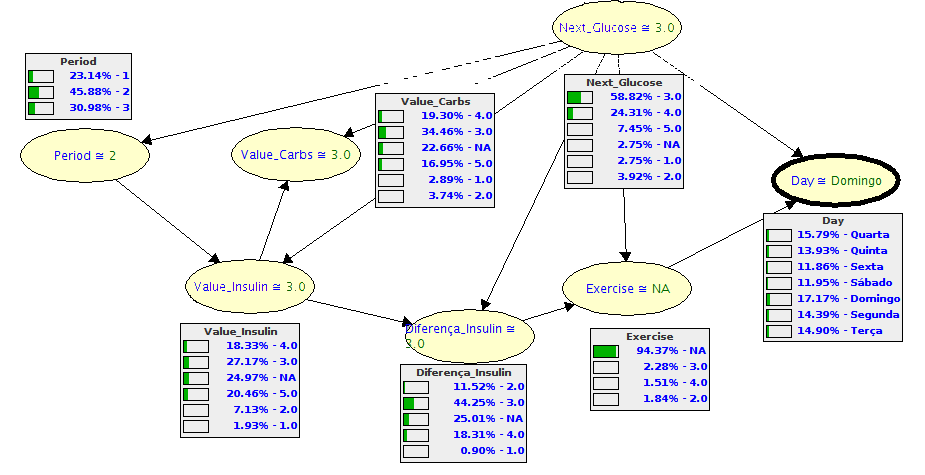
\includegraphics{/home/tiago/Tese/Tese/Databases/CSV/Data/ImagensTese/Utilizador1/Sam.png}
\caption{Glicemia por horas do utilizador 5}
\end{figure}
Para cada variável é possível ver as tabelas de probabilidade para os seus possíveis valores: por exemplo, probabilidades parecidas para os dias da semana indicam que os dias têm uma quantidade de registos parecida. Por sua vez, o valor 3 para glicose tem maior probabilidade que os outros, mostrando que a maioria dos registos de glicemia está dentro dos valores normais.

Podemos ter duas abordagens diferentes: alterar os parâmetros de acordo com as regras de associação geradas, para comprovar a concordância entre os dois programas ou tentar alterar os parâmetros para tentar descobrir padrões que provoquem valores alterados e que não tenham sido descobertos pelas regras. 
Para o primeiro caso, na secção anterior, uma das regras do utilizador 1 mostrava que, às quartas-feiras à tarde, este ingere valores altos de hidratos de carbono pelo que a glicemia tem também valores elevados. No SamIAm, ao selecionar esses três parâmetros com os valores definidos na regra, verifica-se que a probabilidade de ``Next\textunderscore Value=4'' sobe de 24.32\% para 62.68\%, tal como seria de esperar.

Por outro lado, se colocarmos as variáveis de acordo com a regra para hipoglicemia neste utilizador, verificamos que a probabilidade de ``Next\textunderscore Glucose=2'' sobe para 34.74\%.

No entanto, é possível descobrir outros padrões: por exemplo, se selecionarmos apenas o dia ``Domingo'' verificamos que a probabilidade de uma hiperglicemia, ou seja um valor de glicemia 5, sobe para 18.67\%. 

Na figura seguinte pode-se ver quais os parâmetros que provocam uma probabilidade máxima de uma hiperglicemia.

\begin{figure}[H]
\centering
\includegraphics[height=65mm, width=130mm]{/home/tiago/Tese/Tese/Databases/CSV/Data/ImagensTese/Utilizador1/Hiper.png}
\caption{Glicemia por horas do utilizador 5}
\end{figure}
Ou seja, uma nova regra é descoberta: ao Domingo de manhã, quando o utilizador ingere uma quantidade grande de hidratos de carbono, tem maior probabilidade de ter uma hiperglicemia. 

\textbf{Utilizador 2}


A rede para o utilizador 2 é mostrada na figura 6.

\begin{figure}[H]
\centering
\includegraphics[height=65mm, width=130mm]{/home/tiago/Tese/Tese/Databases/CSV/Data/ImagensTese/Utilizador2/Rede.png}
\caption{Glicemia por horas do utilizador 5}
\end{figure}
que, como se verifica, é ligeiramente diferente da rede gerada para o utilizador 1. Uma vez mais, é interessante ver quais os valores dos vários parâmetros que maximizam o valor de glicemia. 

\begin{figure}[H]
\centering
\includegraphics[height=65mm, width=130mm]{/home/tiago/Tese/Tese/Databases/CSV/Data/ImagensTese/Utilizador2/Hiper.png}
\caption{Glicemia por horas do utilizador 5}
\end{figure}
Como se pode observar, a probabilidade de hiperglicemia aumenta bastante aos sábados à tarde, quando o utilizador toma menos insulina que a recomendada. Esta regra não foi gerada pelo algoritmo \textit{apriori}, possivelmente por ter um valor de suporte abaixo do mínimo definido, mas ainda assim é uma regra interessante e que mostra uma utilidade desta análise. É interessante saber quais as condições em que o risco de hiperglicemia é maior, tendo em conta os dados já registados. 

\textbf{Utilizador 3}

A rede criada para o utilizador 3 está representada na figura 6.

\begin{figure}[H]
\centering
\includegraphics[height=65mm, width=130mm]{/home/tiago/Tese/Tese/Databases/CSV/Data/ImagensTese/Utilizador3/Rede.png}
\caption{Glicemia por horas do utilizador 5}
\end{figure}
Esta rede é diferente das redes anteriormente apresentadas. A principal diferença que se nota logo é a falta do nó ``Exercise'' que se deve pelo facto de este utilizador não ter qualquer registo de exercício e portanto, a variável não foi tida em conta. A rede já com as probabilidades é:

\begin{figure}[H]
\centering
\includegraphics[height=65mm, width=130mm]{/home/tiago/Tese/Tese/Databases/CSV/Data/ImagensTese/Utilizador3/Hiper.png}
\caption{Glicemia por horas do utilizador 5}
\end{figure}
Como se pode perceber pela figura 6., este utilizador tem uma probabilidade enorme de ter uma hiperglicemia à terça-feira à tarde, especialmente se tomar menos insulina do que a calculada. 

\textbf{Utilizador 4}

A rede \textit{bayesiana} para o utilizador 4 está representada na figura seguinte, sendo que também é diferente das outras. 

\begin{figure}[H]
\centering
\includegraphics[height=65mm, width=130mm]{/home/tiago/Tese/Tese/Databases/CSV/Data/ImagensTese/Utilizador4/Rede.png}
\caption{Glicemia por horas do utilizador 5}
\end{figure}
Desde logo é possível notar que para a variável ``Insulin\textunderscore Difference'' os valores com probabilidades maiores são o 2 e 4, o que mostra que este utilizador, na maior parte das vezes, toma uma quantidade de insulina diferente da quantidade calculada, o que pode causar consequências nos valores da glicemia. De resto também é possível ver que o exercício é algo raro, tal como nos outros utilizadores. 


\begin{figure}[H]
\centering
\includegraphics[height=65mm, width=130mm]{/home/tiago/Tese/Tese/Databases/CSV/Data/ImagensTese/Utilizador4/Hiper.png}
\caption{Glicemia por horas do utilizador 5}
\end{figure}
Na figura 6. é possível observar que à segunda-feira a probabilidade de ocorrer uma hiperglicemia aumenta consideravelmente, sendo que, neste caso, os outros parâmetros não influenciam muito a probabilidade de hiperglicemia, pelo menos para este dia escolhido. Por exemplo, à segunda-feira a probabilidade de hiperglicemia é parecida para qualquer período.

Por outro lado, verificamos que o utilizador tem uma maior probabilidade de ter um valor de hipoglicemia, isto é, ``Next\textunderscore Glucose=1'' à sexta-feira à tarde, cuja probabilidade aumenta para os 10.19\%.


\textbf{Utilizador 5}


Para o último utilizador, a rede gerada está representada na figura 6.

\begin{figure}[H]
\centering
\includegraphics[height=65mm, width=130mm]{/home/tiago/Tese/Tese/Databases/CSV/Data/ImagensTese/Utilizador5/Rede.png}
\caption{Glicemia por horas do utilizador 5}
\end{figure}
Uma vez mais, um exemplo de uma combinação de parâmetros que aumentam a probabilidade de hiperglicemia é representado na figura 6.

\begin{figure}[H]
\centering
\includegraphics[height=65mm, width=130mm]{/home/tiago/Tese/Tese/Databases/CSV/Data/ImagensTese/Utilizador5/Hiper.png}
\caption{Glicemia por horas do utilizador 5}
\end{figure}
Pela figura 6. é possível notar que à segunda-feira, e quanto o utilizador toma pouca insulina, o valor de glicose no sangue aumenta, ocorrendo uma hiperglicemia. Nesta situação, um simples alerta para aumentar a dose de insulina poderia ser suficiente para corrigir esta situação e acabar com este padrão.

Quanto a hipoglicemias, para este utilizador, a rede mostra que a probabilidade de ``Next\textunderscore Glucose=1'' aumenta nas manhãs em que o utilizador toma mais insulina do que aquela recomendada, sendo que neste caso a probabilidade é de 20.09\%.


\section{\textit{Inductive Logic Programming}}

Para este tipo de análise vamos usar o já mencionado sistema Aleph. Para tal, são necessários três ficheiros: um para exemplos positivos, um para exemplos negativos e outro para o \textit{background knowledge}, sendo que estes três ficheiros teriam de ser em prolog. 
